\begin{figure}[H]
    \centering
    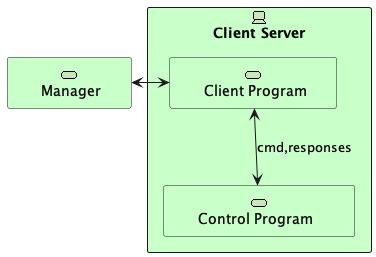
\includegraphics[height=0.3\textheight]{./part/Proyecto_ejecutivo/memoria_descriptiva/descripcionDelProyecto/client/uml/clientServerConcept}
    \caption[Diagrama componentes]{}\label{fig:clientServerConcept}
\end{figure}

\subparagraph{Dominio}

Hay que tener en cuenta que en este programa será casi todo infrestructura. ya que una vez recepcionado el comando mediante el RPC
solo habrá que ejecutarlo en el servidor cliente y será tarea del cliente configurar dicho servidor para que dicho comando exista. Será tarea del programa a ejecutar interpretar dicho comando y trasnformar ese comando y esos argumentos en un dominio interno. Por ejemplo un programa típico de consola en un sistema UNIX

\begin{verbatim}
    ./runMyComand --arg=arg1 --argN=argN
\end{verbatim}


Las posibilidades son tantas como comandos haya instalados en el servidor cliente. En nuestro caso podremos mandar a ejecutar todos los comandos que queramos que vengan previamente instalados en un sistema UNIX y además el programa de control donde podremos interactuar con el motor de corriente continua

\begin{verbatim}
    ./pidControl --velocity=30rpm
    ./pidControl --position=180deg
    ./pidControl --setP=1
    ./pidControl --setI=0
    ./pidControl --setD=0
\end{verbatim}

aquí podemos ver por ejemplo los comándos básicos de un control pid que podremos ejecutar. En la descripción del programa de control y su dominio lo veremos en más detalle


\begin{figure}[H]
    \centering
    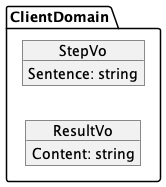
\includegraphics[height=0.4\textheight]{./part/Proyecto_ejecutivo/memoria_descriptiva/descripcionDelProyecto/client/uml/clientDomain}
    \caption[Diagrama de objetos de dominio]{}\label{fig:clientDomain}
\end{figure}

\begin{itemize}
    \item StepDomain
    \begin{itemize}
        \item StepVo
    \end{itemize}
    \item ResultDomain
    \begin{itemize}
        \item ResultVo
    \end{itemize}
\end{itemize}

\subparagraph{casos de uso}

Vamos a describir los casos de uso que podrán ejecutarse en el programa manager. Tenemos 2 Entities y dos aggregate root.

\begin{itemize}
    \item Step
    \item Result
\end{itemize}

\textbf{ejecutar Step}


\subparagraph{estructura de carpetas}

En el proyecto constará de 4 carpetas principales

\tiny
\dirtree{%
    .1 Project .
        .2 Domain.
        .2 Application.
        .2 Adapter.
        .2 Bootstrap.
}
\normalsize

\textbf{Dominio}

\begin{figure}[H]
    \tiny
\dirtree{%
    .1 Domain.
        .2 Step.
            .3 StepVo.
            .3 Repository.
                .4 consoleWrite.
            .3 Services.
                .4 Executor.
        .2 Result.
            .3 ResultVo.
}
\normalsize
    \caption[Diagrama de objetos de dominio]{}\label{fig:1-ClientDomainFolderStructure}
\end{figure}

\textbf{Aplicación}

\tiny
\dirtree{%
.1 Application.
    .2 Port.
        .3 in.
            .4 Step.
                .5 Execute.
                    .6 Command.
                    .6 UseCase.
}
\normalsize

\textbf{Adapters}

\tiny
\dirtree{%
    .1 Adapter.
        .2 in.
            .3 GRPC.
                .4 Harán uso de los useCases de aplicación cuando llegue una request RPC.
            .3 Console.
                .4 Por ejemplo si quisieramos ejecutar los casos de uso mediante terminal.
        .2 out.
            .3 console.
                .4 implementación de los repository de llamada a los servidores clientes.
}
\normalsize





